\chapter{Analyse et spécification des besoins}

\section{Introduction}

Ce chapitre transforme les constats du chapitre précédent en exigences exploitables. Il identifie les acteurs, distingue les besoins fonctionnels et non fonctionnels, formalise les \textbf{règles métier} structurantes, présente les cas d'utilisation puis la traçabilité entre exigences, implémentation et tests. Cette formalisation constitue le socle de la conception.

\section{Étude du processus des urgences}

\subsection{Processus cible}

Le processus cible se décompose en étapes séquentielles et vérifiables :

\begin{enumerate}
    \item \textbf{Enregistrement} : le réceptionniste crée le patient et la visite, fixe la priorité d'enregistrement et le motif ;
    \item \textbf{Triage} : l'infirmier confirme ou ajuste la priorité clinique et l'orientation ;
    \item \textbf{Appel} : le patient est appelé, la file restant ordonnée par priorité puis ancienneté ;
    \item \textbf{Placement} : le patient est affecté à une ressource libre et compatible ;
    \item \textbf{Prise en charge} : le médecin démarre la consultation, la complète et la clôture ;
    \item \textbf{Sortie ou réorientation} : la visite se termine par un outcome (sortie, hospitalisation, transfert), ou le patient est réorienté.
\end{enumerate}

\subsection{Flux d'états}

Pour rendre ce processus informatisable, chaque étape correspond à une transition d'état explicite de la visite. La machine à états est détaillée au chapitre~3 ; elle est la colonne vertébrale du système.

\section{Identification des acteurs}

\begin{table}[H]
\centering
\caption{Acteurs du système et responsabilités}
\label{tab:acteurs}
\small
\begin{tabular}{|l|p{9cm}|}
\hline
\textbf{Acteur} & \textbf{Responsabilités principales} \\
\hline
Réceptionniste & Enregistrer les patients, créer les visites, appeler, déclencher un flag critique. \\
\hline
Infirmier & Trier (priorité P1--P5), placer/retourner, démarrer et compléter la consultation, gérer le cycle des lits, clôturer. \\
\hline
Médecin & Démarrer et clôturer la consultation, remplir le dossier clinique, demander transferts et relèves. \\
\hline
Chef de service & Superviser (SLA, alertes, blocages), administrer les équipes de salle, enregistrer avec override, gérer la capacité. \\
\hline
Administrateur & Gérer les utilisateurs, les rôles et la configuration système et IA. \\
\hline
Patient & Bénéficiaire ; son parcours est suivi et tracé. \\
\hline
Système IA & Assistant optionnel : propose priorité, flux de lits, capacité et documents, sans décider. \\
\hline
\end{tabular}
\end{table}

\section{Besoins fonctionnels}

\subsection{Authentification et gestion des rôles}

Connexion sécurisée par email et mot de passe, génération d'un jeton JWT, contrôle d'accès par rôle et par \textbf{capacités} (par exemple \texttt{register}, \texttt{call}, \texttt{place}, \texttt{triage}, \texttt{close}), gestion du cycle de vie des comptes.

\subsection{Gestion des patients et des visites}

Recherche/création du patient (identification par numéro national), création d'une visite avec code public unique (\texttt{V-AAAAMMJJ-XXXX}), contrainte d'une seule visite active par patient, suivi multi-états (statut, phase de soin, orientation, localisation).

\subsection{File d'attente et appel}

File calculée et non stockée : position déterminée à la lecture par priorité, caractère critique puis ancienneté. L'appel ne retire pas le patient de la file ; il enregistre l'heure d'appel et un compteur d'appels.

\subsection{Triage structuré}

Saisie et historique des évaluations de triage (initiale, réévaluation, escalade) avec priorité P1--P5, note clinique, constantes et orientation ; pose d'un indicateur critique.

\subsection{Gestion des ressources}

Classification des ressources (lit, fauteuil, box, poste de triage, poste de consultation), cycle de vie opérationnel (prêt, nettoyage, maintenance, bloqué, hors service), affectation et libération, historique d'occupation.

\subsection{Prise en charge et consultations}

Démarrage de consultation, attribution du médecin, remplissage du dossier (diagnostic, notes), clôture avec outcome, examens et tâches de soin.

\subsection{Orientation, transferts et relèves}

Demandes de transfert de lit (pendant, confirmé, annulé, expiré) et demandes de relève entre soignants (acceptée, refusée, annulée), avec motif et traçabilité.

\subsection{Supervision et alertes}

Pipeline des patients, détection des blocages (patients « bloqués » au-delà de seuils SLA), alertes opérationnelles hiérarchisées (faible, moyenne, haute, critique) avec acquittement et résolution.

\subsection{Assistance IA}

Recommandations de triage, de flux de lits, de capacité et de documentation, avec traces d'exécution, décisions humaines et approbations.

\section{Besoins non fonctionnels}

\begin{table}[H]
\centering
\caption{Exigences non fonctionnelles}
\label{tab:bnf}
\small
\begin{tabular}{|l|p{9cm}|}
\hline
\textbf{Exigence} & \textbf{Description} \\
\hline
Intégrité & Toute action de visite est atomique (transaction PostgreSQL) ; les contraintes d'intégrité empêchent les états incohérents. \\
\hline
Concurrence & Le verrouillage (\texttt{SELECT ... FOR UPDATE}) empêche deux affectations simultanées du même lit. \\
\hline
Sécurité & JWT, hachage bcrypt, RBAC par capacités, validation serveur, protection des données patients. \\
\hline
Traçabilité & Chaque transition est journalisée dans \texttt{visit\_events} avec acteur, horodatage et métadonnées. \\
\hline
Performance & Réponses API courtes, mises à jour temps réel sans rechargement. \\
\hline
Disponibilité & Service conçu pour un fonctionnement continu (24h/24). \\
\hline
Ergonomie & Tableaux de bord par rôle, interfaces intuitives, thème adapté au rôle. \\
\hline
Évolutivité & Architecture modulaire (services séparés), API REST extensible, migrations versionnées. \\
\hline
Idempotence & Reprise d'action sans doublon grâce à une clé d'idempotence. \\
\hline
\end{tabular}
\end{table}

\section{Règles métier structurantes}

Les règles suivantes gouvernent la cohérence du système et sont appliquées côté serveur, jamais uniquement côté interface :

\begin{enumerate}
    \item \textbf{Une seule visite active par patient} ; un patient n'a jamais deux prises en charge ouvertes.
    \item \textbf{Une seule affectation active par visite} et \textbf{un seul patient par ressource}.
    \item \textbf{Transitions autorisées uniquement} : une action invalide pour l'état courant est rejetée (code HTTP~400/409).
    \item \textbf{Compatibilité des ressources} : une ressource en nettoyage, maintenance, bloquée ou hors service ne peut être affectée.
    \item \textbf{Tri obligatoire avant prise en charge} : la phase de soin suit une phase de triage explicite.
    \item \textbf{Décision clinique humaine} : le triage et la clôture clinique ne sont jamais automatiques.
    \item \textbf{Approbation humaine des actions IA} : toute action IA à risque exige une approbation, sauf outils explicitement autorisés.
\end{enumerate}

\section{Diagramme de cas d'utilisation}

\begin{figure}[H]
    \centering
    % Image à déposer dans rapport-stage/images/ : use_case_diagram.png
    \IfFileExists{images/use_case_diagram.png}{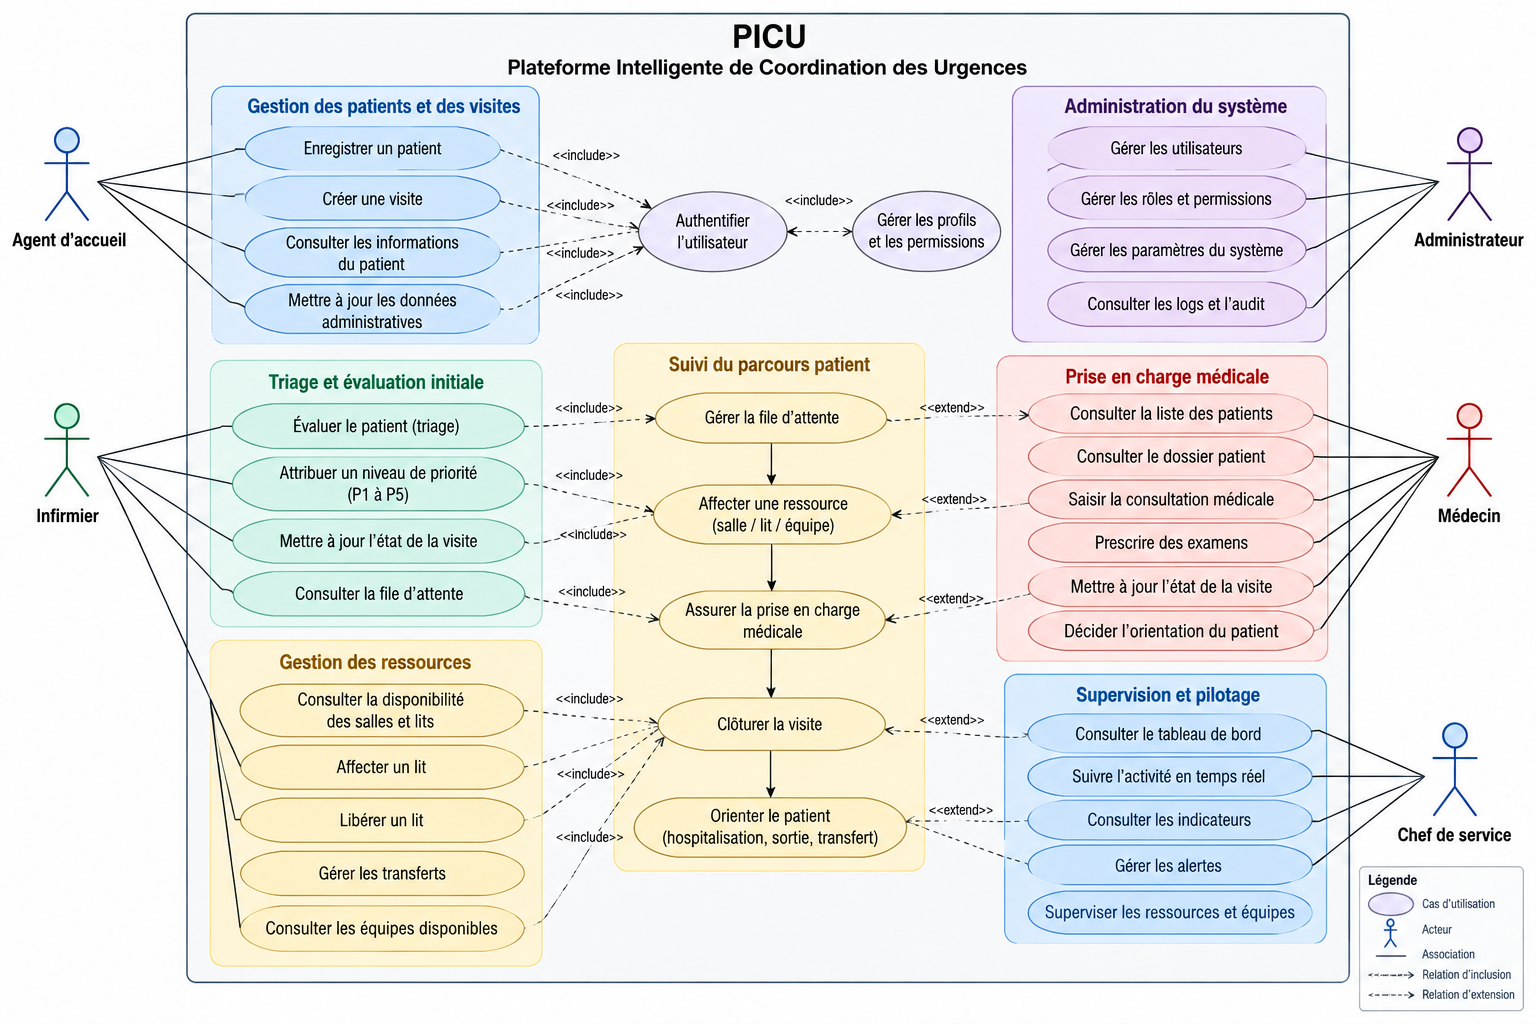
\includegraphics[width=0.9\textwidth]{images/use_case_diagram.png}}{\fbox{\parbox{0.9\textwidth}{\centering\vspace{1.5cm}À insérer : \texttt{images/use\_case\_diagram.png}\vspace{1.5cm}}}}
    \caption{Diagramme de cas d'utilisation de PICU}
    \label{fig:use_case_diagram}
\end{figure}

\section{Description des principaux cas d'utilisation}

\subsubsection{UC1 — Authentification et redirection par rôle}
\textbf{Acteur} : tous. Connexion par identifiants, émission d'un jeton JWT, redirection vers le tableau de bord du rôle.

\subsubsection{UC2 — Enregistrement d'un patient}
\textbf{Acteur} : Réceptionniste, Chef. Recherche par numéro national, création du patient et de la visite, priorité d'enregistrement et motif ; la visite entre en phase \texttt{triage\_pending}.

\subsubsection{UC3 — Triage clinique}
\textbf{Acteur} : Infirmier. Saisie d'une évaluation de triage (priorité, note, constantes, orientation), historique conservé.

\subsubsection{UC4 — Appel et placement}
\textbf{Acteur} : Réceptionniste, Infirmier. Appel du patient dans la file, puis affectation à une ressource compatible et libre.

\subsubsection{UC5 — Prise en charge médicale}
\textbf{Acteur} : Médecin, Infirmier. Démarrage de consultation, remplissage du dossier, clôture avec outcome.

\subsubsection{UC6 — Transfert et relève}
\textbf{Acteur} : Médecin, Infirmier, Chef. Demande de transfert de lit ou de relève, confirmée ou refusée selon les rôles autorisés.

\subsubsection{UC7 — Supervision}
\textbf{Acteur} : Chef. Consultation du pipeline, des indicateurs SLA et des alertes opérationnelles ; acquittement et résolution.

\subsubsection{UC8 — Assistance IA}
\textbf{Acteur} : Système IA, personnel habilité. Production de recommandations et, le cas échéant, proposition d'actions soumises à approbation.

\subsubsection{UC9 — Administration}
\textbf{Acteur} : Administrateur. Gestion des utilisateurs, des rôles et de la configuration (dont les paramètres IA).

\section{Matrice de traçabilité des exigences}

La rigueur d'ingénierie exige de relier chaque exigence à son implémentation et à sa validation. Le tableau suivant en donne un extrait (la matrice complète figure en annexe).

\begin{table}[H]
\centering
\caption{Extrait de la matrice Exigence $\rightarrow$ Implémentation $\rightarrow$ Test}
\label{tab:matrice}
\small
\begin{tabular}{|l|l|l|}
\hline
\textbf{Exigence} & \textbf{Implémentation} & \textbf{Validation} \\
\hline
Une seule visite active & \texttt{visitService.registerVisit} & Test d'intégrité / 409 \\
\hline
Un seul patient par lit & \texttt{assertBedAssignable}, verrou & Test concurrence / 409 \\
\hline
Transitions valides & \texttt{visitService}, \texttt{careStage} & Tests par rôle \\
\hline
Lit non affectable si « cleaning » & \texttt{resourceService} & \texttt{npm run test:v4} \\
\hline
Seuils SLA non approuvés inactifs & \texttt{supervisionRulesService} & \texttt{npm run test:supervision} \\
\hline
Indices d'enregistrement & \texttt{registrationHints} & \texttt{npm run test:registration} \\
\hline
Actions IA à risque approuvées & \texttt{action-policy} & Tests de politique IA \\
\hline
\end{tabular}
\end{table}

\section{Gestion des risques}

\begin{table}[H]
\centering
\caption{Risques identifiés et mesures de prévention}
\label{tab:risques}
\small
\begin{tabular}{|p{3.4cm}|p{5.6cm}|p{4.4cm}|}
\hline
\textbf{Risque} & \textbf{Mesure de prévention} & \textbf{Limite résiduelle} \\
\hline
Erreur de priorisation & Assistance IA supervisée + historique de triage & Précision IA perfectible \\
\hline
Conflit d'affectation d'un lit & Verrou \texttt{FOR UPDATE} + contrainte d'affectation unique & Dépend de la disponibilité réelle \\
\hline
Perte de connexion temps réel & Raisonnement par état serveur + rechargement & Latence possible des écrans \\
\hline
Confidentialité des données & RBAC, JWT, secrets hors dépôt & Pas d'audit externe réalisé \\
\hline
Décision automatisée abusive & Politique d'actions IA, approbation obligatoire, mode simulation restreint & Nécessite gouvernance continue \\
\hline
\end{tabular}
\end{table}

\section{Conclusion}

Les besoins sont formalisés en exigences fonctionnelles et non fonctionnelles, règles métier, cas d'utilisation, matrice de traçabilité et analyse de risques. Le chapitre suivant présente la méthodologie de développement et la conception du système.
